\setAuthor{Jaan Kalda}
\setRound{piirkonnavoor}
\setYear{2022}
\setNumber{G 8}
\setDifficulty{8}
\setTopic{TODO}

\prob{Tühi pudel}
Kokapoiss peseb liitrist plastpudelit: laseb sinna natuke kuuma vett temperatuuril $t_v=\qty{55}{\celsius}$, suleb pöidlaga pudelikaela ja raputab tugevasti. Kui ta pöidla nüüd pudeli suu eest ära võtab, käib väike plaksatus ja pudelist surub veidi õhku välja, sest rõhk pudelis oli suurem atmosfäärirõhust. Kui suur oli rõhkude vahe? Toas on õhutemperatuur $t_t=\qty{20}{\celsius}$, suhteline õhuniiskus $r=\qty{50}{\percent}$ ja õhurõhk $p_0=\SI{1.01e5}{Pa}$? Küllastunud veeauru rõhu sõltuvus temperatuurist on toodud juuresoleval graafikul.
\begin{figure}[h]
  \vspace{-0.5em}
  {
    \tikzset{component/.style={draw,thick,circle,fill=white,minimum size=0.75cm,inner sep=0pt}}
    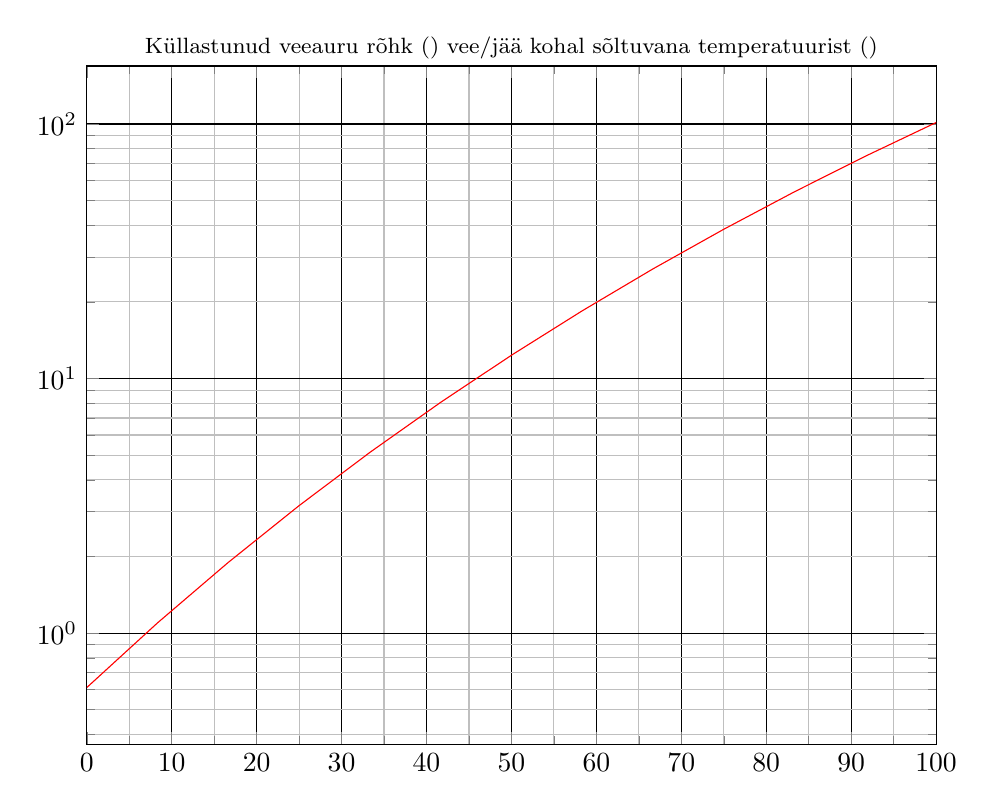
\begin{tikzpicture}
      \begin{axis}[
        ymode=log,
        width=1.02\textwidth,
        height=29em,
        minor tick num=1,
        major grid style = black,
        grid=both,
        % xlabel=$t$ (\unit{\celsius}),
        % ylabel=$P$ (\unit{\kPa}),
        xmin = 0, xmax = 100,
        title={\footnotesize Küllastunud veeauru rõhk (\unit{\kPa}) vee/jää kohal sõltuvana temperatuurist (\unit{\celsius})},
        title style={xshift=0, yshift=-7pt},
        ]
        \addplot[red, domain=0:200] {0.61121*exp((18.678-x/234.5)*(x/(257.14+x)))};
        \addplot[blue, domain=-200:0] {0.61115*exp((23.036-x/333.7)*(x/(279.82+x)))};
      \end{axis}
    \end{tikzpicture}
  }
  \vspace{-1em}
\end{figure}


\hint

\solu
Rõhk pudelis kasvab kahel põhjusel. Esiteks, toimub pudelisse suletud õhu (va veeauru molekulid) isohooriline paisumine toatemperatuurilt kuni vee tempreatuurini --- võime eeldada, et raputamise käigus annab vesi soojust õhule ning vee soojusmahtuvus on nii suur, et see ei jõua oluliselt jahtuda \p1. Teiseks kasvab õhus veeauru osarõhk, korraliku raputamise tulemusel saabub pudelisse termodünaamiline tasakaal, mis tähendab, et pudelis oleva õhu temperatuur võrdub vee temperatuuriga ja veeauru rõhk võrdub küllastunud auru rõhuga antud temperatuuril \p1.

Esimese komponendi leidmiseks paneme tähele, et enne raputamist oli õhu osarõhk pudelis (õhu rõhk ilma veeauru rõhuta) $p_0'=p_0-rp_k(\qty{20}\celsius)\approx p_0$, sest veeauru osarõhk on palju väiksem atmosfäärirõhust. Avaldis õhu osarõhu jaoks pudelis enne loksutamist, olgu see siis täpne või lihtsustatult $p_0$, annab \p1; selle punkti saab kätte ka siis, kui õpilane kasutab ilma pikemalt põhjendamata järgnevas isohoori seaduses atmosfäärirõhku $p_0$). Eelnevas avaldises esines auru rõhu osarõhk toaõhus $p_a=rp_k(\qty{20}\celsius)$ \p1, mille väärtust läheb hiljem vaja.  Selle arvuliseks leidmiseks tuleb võtta graafikult lugem küllastunud auru rõhu jaoks, $p_k(\qty{20}\celsius)\approx \qty{2.2}{\kPa}$; täpne lugem (väärtused vahemikus $\qty{2.2\pm 0.1}{\kPa}$) annab \p1 ja vähem täpne lugem (väärtused vahemikus $\qty{2.2\pm 0.2}{\kPa}$) annab \p{0,5} (suurema vea korral punkte ei saa). Ideaalse gaasi olekuvõrrandist teame, et konstantsel ruumalal on rõhk võrdeline temperatuuriga, seega uus õhu osarõhk $p_1= p_0T_v/T_t$ \p1 ning järelikult vastav rõhu kasv pudeli sees $\Delta p_1\equiv p_1-p_0=p_0'(T_v/T_t-1)\approx \SI{12}{\kPa}$ (avaldis $\Delta p_1$ jaoks annab \p1 ja õige numbriline väärtus \p1), kus temperatuurid on esitatud Kelvinites.

Teise komponendi leiame kui veeauru rõhkude vahe: $\Delta p_2 = p_k(\qty{55}{\celsius}) - \num{0.5}p_k(\qty{20}{\celsius}) \approx \SI{15}{\kPa} -\num{0.5}\cdot\qty{2.2}{\kPa}\approx \qty{14}{\kPa}$. Idee eest avaldada veeauru osarõhu muutus graafikult loetavate rõhkude vahena annab \p1; $p_k(\SI{55}\celsius)$ korrektne leidmine graafikult (väärtused vahemikus $\SI{1.5\pm 0.1}{kPa}$)  annab veel \p1 (suurema vea korral saab vahemiku $\SI{1.5\pm 0.2}{kPa}$ korral \p{0,5}).

Seega oli rõhk pudelis $\approx \SI{25}{kPa}$ võrra suurem, kui toas.
\probend